% !TEX root = ../main.tex
\chapter{PHÂN TÍCH THIẾT KẾ HỆ THỐNG}

\section{Mục 2.1}
Mô tả kiến trúc tổng quan của hệ thống bài tập lớn.

\subsection{Mục 2.1.1}
Sơ đồ kiến trúc và luồng dữ liệu của ứng dụng.

\begin{figure}[htbp]
  \centering
  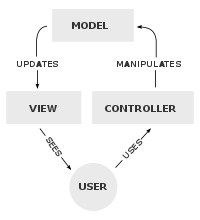
\includegraphics[width=0.6\textwidth]{sample_img.png}
  \caption{Hình ảnh mẫu sơ đồ hệ thống}
  \label{fig:sample}
\end{figure}

Như được thể hiện trên Hình \ref{fig:sample}, hệ thống gồm các thành phần cơ bản xử lý từ đầu vào đến kết quả trả về.

\subsection{Mục 2.1.2}
Phân tích thiết kế Cơ sở dữ liệu và các thành phần giao tiếp API.
